%% 
%% Copyright 2019-2021 Elsevier Ltd
%% 
%% This file is part of the 'CAS Bundle'.
%% --------------------------------------
%% 
%% It may be distributed under the conditions of the LaTeX Project Public
%% License, either version 1.2 of this license or (at your option) any
%% later version.  The latest version of this license is in
%%    http://www.latex-project.org/lppl.txt
%% and version 1.2 or later is part of all distributions of LaTeX
%% version 1999/12/01 or later.
%% 
%% The list of all files belonging to the 'CAS Bundle' is
%% given in the file `manifest.txt'.
%% 
%% Template article for cas-dc documentclass for 
%% double column output.

\documentclass[fleqn]{cas-sc}

\usepackage{lipsum}
\usepackage{tikz}
\usetikzlibrary{shapes, snakes, calc}

% If the frontmatter runs over more than one page
% use the longmktitle option.

%\documentclass[a4paper,fleqn,longmktitle]{cas-dc}

%\usepackage[numbers]{natbib}
%\usepackage[authoryear]{natbib}
\usepackage[authoryear,longnamesfirst]{natbib}

%%%Author macros
\def\tsc#1{\csdef{#1}{\textsc{\lowercase{#1}}\xspace}}
\tsc{WGM}
\tsc{QE}
%%%

% Uncomment and use as if needed
%\newtheorem{theorem}{Theorem}
%\newtheorem{lemma}[theorem]{Lemma}
%\newdefinition{rmk}{Remark}
%\newproof{pf}{Proof}
%\newproof{pot}{Proof of Theorem \ref{thm}}

\begin{document}
\let\WriteBookmarks\relax
\def\floatpagepagefraction{1}
\def\textpagefraction{.001}

% Short title
\shorttitle{Ambulance Dispatch}    

% Short author
\shortauthors{Burkman, Jin, Abuhijleh, and Sun}  

% Main title of the paper
\title [mode = title]{Modeling the Need for an Ambulance based on Automated Crash Reports from iPhones}  

% Title footnote mark
% eg: \tnotemark[1]
%\tnotemark[<tnote number>] 
%\tnotemark[1] 

% Title footnote 1.
% eg: \tnotetext[1]{Title footnote text}
%\tnotetext[1]{Working Title} 

% First author
%
% Options: Use if required
% eg: \author[1,3]{Author Name}[type=editor,
%       style=chinese,
%       auid=000,
%       bioid=1,
%       prefix=Sir,
%       orcid=0000-0000-0000-0000,
%       facebook=<facebook id>,
%       twitter=<twitter id>,
%       linkedin=<linkedin id>,
%       gplus=<gplus id>]

%\author[<aff no>]{<author name>}[<options>]
\author[1,2]{J. Bradford Burkman}[]
% Footnote of the first author
%\fnmark[1]
% Corresponding author indication
%\cormark[1]
% Email id of the first author
\ead{bradburkman@gmail.com}
% URL of the first author
\ead[url]{http://www.github.com/bburkman}

% Credit authorship
% eg: \credit{Conceptualization of this study, Methodology, Software}
% Options: conceptualization; data curation; formal analysis; funding acquisition; investigation; methodology; project administration; resources; software; supervision; validation; visualization; writing – original draft; and writing – review and editing.
\credit{Conceptualization, Investigation, Writing - original draft, Visualization}


\author[1]{Miao Jin}[]
\credit{Supervision, Methodology, Writing - review and editing}

\author[1,3]{Malek Abuhijleh}[]
\credit{Investigation, Methodology}

\author[3]{Xiaoduan Sun}[]
\credit{Data curation, Writing - review and editing}






\affiliation[1]{organization={School of Computing and Informatics, University of Louisiana at Lafayette},
%            addressline={301 E. Lewis St}, 
%            city={Lafayette},
%          citysep={}, % Uncomment if no comma needed between city and postcode
%            state={LA},
%            postcode={70503}, 
            country={USA}}

% Address/affiliation
\affiliation[2]{organization={Louisiana School for Math, Science, and the Arts},
%            addressline={715 University Pkwy}, 
%            city={Natchitoches},
%          citysep={}, % Uncomment if no comma needed between city and postcode
%            state={LA},
%            postcode={71457}, 
            country={USA}}

\affiliation[3]{organization={Department of Civil Engineering, University of Louisiana at Lafayette},
%            addressline={131 Rex St}, 
%            city={Lafayette},
%          citysep={}, % Uncomment if no comma needed between city and postcode
%            state={LA},
%            postcode={70504}, 
            country={USA}}




% For a title note without a number/mark
%\nonumnote{}

% Here goes the abstract
\begin{abstract}
%%%%% Abstract
% I found an abstract in TRpC June 2022 with 365 words.
Put abstract here.
\vskip 1in

\end{abstract}

% Use if graphical abstract is present
%\begin{graphicalabstract}
%\includegraphics{}
%\end{graphicalabstract}

% Research highlights
\begin{highlights}
	\item  Supports transferability and benchmarking of different approaches on a public large-scale dataset.  The associated GitHub page provides the code and detailed notes used to perform the analysis on the Crash Report Sampling System.  
	\item Novel Application motivated by Emerging Technology:  Machine Learning Classification Models for Dispatching Ambulances based on Automated Crash Reports
	\item New Use of Dataset:  Used Crash Report Sampling System (CRSS), which has imputed missing values for some features, but not all of the ones we wanted to use.  For the first time we have seen, we used the software the CRSS authors use for multiple imputation (IVEware) to impute missing values in more features.  
	\item Perennial Machine Learning Challenge:  Imbalanced Datasets.
\end{highlights}

% Keywords
% Each keyword is seperated by \sep
\begin{keywords}
 \sep Automated crash notification \sep Ambulance dispatch \sep Emergency medical services  \sep Machine learning
\end{keywords}

\maketitle

% Main text

%%%%% Introduction
\section{Introduction}\label{What does the label do?}

\begin{comment}
	Notes from 5/16/22 meeting with Dr. Jin:
		I Motivation - Good, needs more material
		II Analyze Difficulty in Solving Problem
		III ML/Data Analysis
			Tradeoffs
			Limits of Methods
		IV Plan
		
		Mention overlaps with other work
\end{comment}

%%%
\subsection{Motivation}


%Starting in 2022, each new iPhone has a feature that can automatically notify police if the phone detects the deceleration profile of a crash.  If the injuries are serious, time to medical care is critical, but few crashes result in serious injuries, and ambulances are in limited supply and expensive.  From the data available from such an automatic notification, can we build a machine-learning model that will recommend whether police should immediately, perhaps automatically, dispatch an ambulance?  

A Google Pixel phone can detect the deceleration profile of a car crash and, if you have enabled the settings in the Personal Safety app, will, if you do not respond in 60 seconds, automatically call the police, reporting your location.  Apple announced in November 2021 that it was planning to do something similar.  

The crash victims who would most obviously benefit from such technology are those in crashes with no witnesses to call police (``unnoticed run-off roadway''), who survived the crash and might have lived if help had arrived promptly, but died from their injuries.  Such crashes are very rare, about seventy-seven fatalities annually in the US in 2010-2018,   
\citep{SPICER2021105974}
of the about 35,000 crash fatalities per year in the same time period.  \citep{FARS}
% 2020:  38,824
% 2019:  36,355
% 2018:  36,835
% 2017:  37,473
% 2016:  37,806
% 2015:  35,484
% 2014:  32,744
% 2013:  32,893
% 2012:  33,782
% 2011:  32,479
% 2010:  32,999

A much larger group who could benefit from faster ambulance response are those injuries are serious and need prompt medical attention.  Dispatching an ambulance automatically, rather than waiting for an eyewitness to call for one, would cut at least several minutes off of the ambulance response time.  In a 1996 study on 1990 data for US urban interstates, freeways, and expressways \citep{edsoai.on1047979037n.d.}, the average accident notification time was 5.2 minutes, and the additional time to EMS (emergency medical services) arrival was 6.2 minutes.    Evanco estimated that reducing the notification time from 5.2 minutes to 2 minutes would cut fatalities by 15.9\%.   Even those who might not die may recover more fully and quickly with prompt medical attention, so dispatching an ambulance promptly when one is needed would be beneficial.  

On the other hand, we do not want to send an ambulance to every accident scene, because only a small proportion of crashes have severe injury; most are property damage only (PDO) crashes.  Ambulances and their crews are expensive and in finite supply.  

{\bf [Insert cost differential discussion]}

Given the information available to the police from a phone's automated crash notification, can we build a model that will recommend (or determine) whether to send an ambulance immediately?  





%%%
\subsection{Difficulty in Solving Problem}

Such a model will not be perfect, with some false negatives (not sending an ambulance when one is needed) and many false positives (sending an ambulance when one is not needed).  We will show that the quality of the model depends largely on what information is available.  Some information (location, time of day, day of week, weather) either comes with the automated report or is easy to get.  Other information (age and sex of phone's primary user, vehicle likely to be driven by that person) may be very helpful in predicting injury, but getting that information would require instantaneous communication between private and public databases.  Being able to interpret the location, ({\it e.g.} Is that precise location inside an intersection of two roads with high speed limits?) in real time would require planning and preparation.  

The problem is both political and ethical as well as technical.  How many false positives will we tolerate to have one fewer false negative?  We will show that, given such a marginal tolerance $p$, we can incorporate that tradeoff into the model, but each locality will have to decide that for itself.  Implementing such a system would require budgets, cooperation, and possibly legislation, but knowing which data is most useful can help set priorities.  



%%%
\subsection{Machine Learning Challenges}

We deal with several machine learning challenges in our study, and their solutions are often as much art as science.  

\begin{description}

	\item [Two Datasets]  
	
For this study we used two datasets, the US Department of Transportation's  National Highway Transportation Safety Administration (NHTSA)'s Crash Report Sampling System (CRSS) 2016-2020 and a census of crash reports in Louisiana 2014-2018. \citep{CRSS}  Both datasets record about five hundred thousand crashes, with details on the crash and on each vehicle and each person involved.  The two datasets are similarly structured.  

We will look at the data at the level of each person involved in a crash (``crash person''), as each automated crash notification corresponds to a phone, which corresponds to a person.  	
	
The major difference between the two datasets is that, while the Louisiana is a census (all police crash reports), the CRSS is sample that intentionally over-represents more serious crashes.   In the Louisiana data, 8.5\% of the crash persons were transported to a hospital, while in the CRSS sample, it's 16.1\%.  
Comparing the results will require interpretation and justification.
	
	\item [Feature Selection and Engineering]  We need to select the features most relevant to crash severity; too many less-relevant features will muddle the model building.  CRSS has both ``Make'' and ``Body Type.''  Do these two features give enough different information that we should use both?  If not, which is more useful?
	
Some features have many values that we can usefully combine into bins or bands.  For instance, CRSS has ninety-seven different categories of vehicle body type, and our model building would work better if we could condense those to fewer than ten categories.  Is a compact pickup truck more like a car or a standard pickup?  We look at the likelihood that a crash vehicle's occupants require transportation to a hospital when making such classification decisions, and classify the compact pickup truck with the cars.  

The \verb|AGE| feature has values 0-120.   A simple approach would be to put it in decade bands, but in most states in the US, the driving age is 16.  The crash severity profiles for new drivers are different than for experienced drivers, so a split at 15/16 makes sense.  In our analysis, the crash severity profiles for ages 52-70 are similar to each other but different from 71+, so we broke them into bands there.  
	
We can also merge features into useful new features.  In both data sets, we have ``Day of Week'' and ``Hour.''  We would like to take from each to make ``Rush Hour,'' if it has a different hospitalization profile.  When does it start and end?  Is morning rush hour different from evening?  Does it start earlier on Fridays?  
	
	\item [Missing Data]  As with all real data, many samples (records) have missing values.  The Louisiana data is raw, with many values listed as ``unknown.'' For many features (fields, columns) of the CRSS, the authors have created another feature with the missing values imputed.  Trusting that those authors understand the data better than we do and may have access to redacted data, we use the imputed features.  For the Louisiana data, we will have to impute, delete, or ignore missing data; again, as much art as science.  

	
\end{description}



%%%
\subsection{Imbalanced Data}

Only a small proportion of crashes require immediate medical attention.  In the CRSS data, about 15\% of persons involved in a crash were transported by ambulance.  If we built a model that classified all crashes as ``Ambulance Not Needed,'' the model would have 85\% accuracy, which would be excellent in some other applications, but not here.  The toolkit for building models on imbalanced data is well established, but many of the tools only work for continuous data (our data is all categorical).
	 

%%%
\subsection{Research Plan}

\begin{enumerate}
	\item On both raw data sets, do cleanup, feature selection, and feature engineering.  To the extent possible, make the two engineered data sets the same.
	\item Starting with the easiest-to-obtain data (general location, time/day, weather), and interatively adding more data (persons, vehicles, specific location), build and evaluate a model that predicts whether an ambulance is needed.
	\item Combine results from the two datasets.
	\item Interpret and discuss how the model improves as more data becomes available.  
\end{enumerate}

%%%%% Lit Review
\section{Literature Review}
%%%
\subsection{Apps to Detect Crashes}
The idea of using the accelerometer in a cell phone to detect a crash and notify the police goes back to at least 2011 with {\it WreckWatch}, an app prototype by \cite{RN29097389220110101}.  A few years later, \cite{edseee.692210720140801} proposed an app that would detect not only a crash but its severity, and send the phone owner's medical information.  In September 2019, Google hinted that it would have crash detection in its Pixel phones soon \citep{XDA}, and it is now available \citep{GooglePixelCrash}.  In November 2021, the Wall Street Journal announced that Apple was thinking of introducing such an app in its iPhones and Apple watches in 2022 \cite{edsgcl.68102971120211102}, but as of this writing, such an app had not come out yet.  The App Store does have some unverified third-party apps, like those from \cite{SOSmart} and \cite{Blink!}.


%%%
\subsection{Imbalanced Data}

In building a model to predict, based on records of roadside inspections, traffic violations, and previous crashes, future crashes for trucks, \cite{LACK2021106105} described the imbalanced data problem well.

\begin{quote}
Initial models ``correctly'' classified no-crash versus crash instances 99\% of the time, but almost never correctly predicting a crash—a major failure in achieving the goal of this analysis and a common issue in unbalanced datasets.
\end{quote}


Our work in this paper uses the most straightforward of machine learning (ML) algorithms, the binary classifier.  We want to answer, ``Should we send an ambulance to this crash,'' and are using historical data answering for each crash, ``Did we use an ambulance?''  We want to build a model that will look at the data we have for a crash and return a prediction.  To build it, we will separate our data into a training set and a test set; use the training set to build the model, then evaluate the model on the (unseen during model building) test set.  

The model will not be perfect.  We want to send ambulances to all of the crashes that need one (True Positive), and not send ambulances to crashes that don't (True Negative).  Sending an ambulance when one is not needed (False Positive) is unnecessarily expensive, but if we don't send an ambulance when one is needed (False Negative), someone might die unnecessarily.

We can visually organize the success and failures of our binary classification model in a {\it confusion matrix} (also called {\it error matrix}, or {\it contingency table}).


\begin{center}
\begin{tabular}{cc|c|c|}
	&\multicolumn{1}{c}{}& \multicolumn{2}{c}{Prediction} \cr
	&\multicolumn{1}{c}{} & \multicolumn{1}{c}{N} & \multicolumn{1}{c}{P} \cr\cline{3-4}
	\multirow{2}{*}{Actual}&N & TN & FP \vrule width 0pt height 10pt depth 2pt \cr\cline{3-4}
	&P & FN & TP \vrule width 0pt height 10pt depth 2pt \cr\cline{3-4}
\end{tabular}
\end{center}

Most machine learning algorithms are designed to maximize {\it accuracy}, the proportion of classifications that were successful.  

$$\text{Accuracy} = \frac{ \text{TN} + \text{TP}}{\text{TN} + \text{FP} + \text{FN} + \text{TP}}$$

In many applications, the accuracy is straightforward and useful, but not if the data are imbalanced.  In our case, in all of the reported crashes in Louisiana in 2014-2018, there were 645,748 people involved in the crashes, and 55,164 used an ambulance (\verb|OCC_MED_TRANS_CD = A|), 8.5\% of the total.  

If we built a model that predicted that none of the crashes required an ambulance, our model would have 91.5\% accuracy.  


\

\hfil \begin{tabular}{cc|c|c|}
	&\multicolumn{1}{c}{}& \multicolumn{2}{c}{Prediction} \cr
	&\multicolumn{1}{c}{} & \multicolumn{1}{c}{N} & \multicolumn{1}{c}{P} \cr\cline{3-4}
	\multirow{2}{*}{Actual}&N & 590,584 & 0 \vrule width 0pt height 10pt depth 2pt \cr\cline{3-4}
	&P & 55,164 & 0 \vrule width 0pt height 10pt depth 2pt \cr\cline{3-4}
\end{tabular}

\

$$\text{Accuracy} = \frac{ \text{590,584} + \text{0}}{\text{590,584} + \text{0} + \text{55,164} + \text{0}} \approx 0.915$$

In many applications, 91\% accuracy would be good.  Why is it different in our context?  For two reasons.  First, our model is useless because we have entirely misclassified all of the positive samples.  Second, accuracy gives the same weight to false positives and false negatives, but in our application, their costs are very different.  The cost of a false positive (sending an ambulance when one is not necessary) is measured in money, while the cost of a false negative (not sending an ambulance promptly when one is necessary) is measured in lives.  We are willing to trade off sending $p$ number of unnecessary ambulances if it means that we will send one more necessary ambulance.  [Choosing the value of $p$ is a question for ethicists and politicians that we will discuss later.]

There are four [citation] categories of methods for building a machine learning model on an imbalanced dataset, and we will use all four in this paper.  

\begin{itemize}
	\item Data-level techniques to artificially balance the dataset
	\item Modifying the loss function in building the model
	\item Modifying the model-building algorithm
	\item Changing the metric in evaluating the model
\end{itemize}

%%%
\subsection{Data-Level Techniques for Imbalanced Data}

Consider this two-dimensional training dataset, which we will use to illustrate data-level techniques for handling imbalanced datasets.    The six circles represent samples (elements) of the majority negative class (``no ambulance''), and the three squares represent the minority positive class (``ambulance'').  


\begin{center}
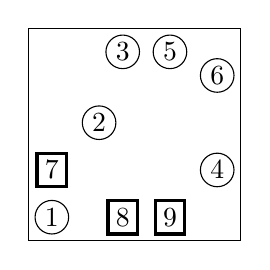
\begin{tikzpicture}[x = 3mm, y=3mm]
	\draw (-1,-1) rectangle (8,8);
	\tikzstyle{Square} = [
		draw, 
		very thick,
		rectangle,
		inner sep = 1mm,
		minimum size = 2 mm
	]
	\tikzstyle{SquareFill} = [
		draw, 
%		fill = black,
		very thick,
		rectangle,
	]
	\tikzstyle{Circle} = [
		draw, 
		circle,		
		inner sep = 0.5mm,
	]
	\tikzstyle{CircleFill} = [
		draw,
%		fill = blue, 
		circle,
	]
	\node [Circle] (1) at (0,0) {1};
	\node [Circle] (2) at (2,4) {2};
	\node [Circle] (3) at (3,7) {3};
	\node [Circle] (4) at (7,2) {4};
	\node [Circle] (5) at (5,7) {5};
	\node [Circle] (6) at (7,6) {6};
	\node [Square] (7) at (0,2) {7};
	\node [Square] (8) at (3,0) {8};
	\node [Square] (9) at (5,0) {9};

\end{tikzpicture}
\end{center}

Many algorithms have been proposed to balance the two classes before applying a machine learning algorithm to build a model to classify new samples as positive or negative.  %WARNING:  Vast oversimplification ahead.  Our goal here is to give the general idea of each method.  



\subsubsection{Random Undersampling}

Random undersampling balances the two classes by randomly deleting elements of the majority class until the two are balanced.  The major drawback of this method is that you throw away information about the majority class.  If the majority class is many more times the size of the minority, you lose almost all of the data.  


\begin{center}
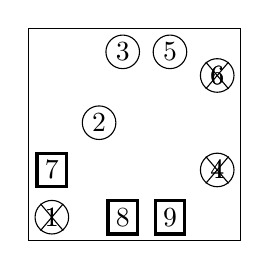
\begin{tikzpicture}[x = 3mm, y=3mm]
	\draw (-1,-1) rectangle (8,8);
	\tikzstyle{Square} = [
		draw, 
		very thick,
		rectangle,
		inner sep = 1 mm,
		minimum size = 3 mm
	]
	\tikzstyle{SquareFill} = [
		draw, 
		fill = black,
		very thick,
		rectangle,
	]
	\tikzstyle{Circle} = [
		draw, 
		circle,
		inner sep = 0.5 mm
	]
	\tikzstyle{CircleFill} = [
		draw,
		fill = blue, 
		circle,
	]
	\node [Circle] (1) at (0,0) {1};
	\node [Circle] (2) at (2,4) {2};
	\node [Circle] (3) at (3,7) {3};
	\node [Circle] (4) at (7,2) {4};
	\node [Circle] (5) at (5,7) {5};
	\node [Circle] (6) at (7,6) {6};
	\node [Square] (7) at (0,2) {7};
	\node [Square] (8) at (3,0) {8};
	\node [Square] (9) at (5,0) {9};

	\node [Circle, cross out] (1) at (0,0) {1};
	\node [Circle, cross out] (4) at (7,2) {4};
	\node [Circle, cross out] (6) at (7,6) {6};
\end{tikzpicture}
\end{center}

Bagging algorithms use random undersampling multiple times, building multiple models with different undersamplings then aggregating the results.  

\subsubsection{Random Oversampling}

Random oversampling creates duplicates of minority class samples until the sets are balanced.  This method has a similar effect to using class weights, introduced below.  

\begin{center}
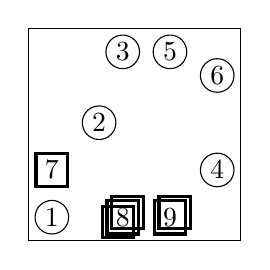
\begin{tikzpicture}[x = 3mm, y=3mm]
	\draw (-1,-1) rectangle (8,8);
	\tikzstyle{Square} = [
		draw, 
		very thick,
		rectangle,
		inner sep = 1mm,
		minimum size = 4 mm
	]
	\tikzstyle{SquareFill} = [
		draw, 
		fill = black,`	
		very thick,
		rectangle,
	]
	\tikzstyle{Circle} = [
		draw, 
		circle,
		inner sep = 0.5 mm
	]
	\tikzstyle{CircleFill} = [
		draw,
		fill = blue, 
		circle,
	]
	\node [Circle] (1) at (0,0) {1};
	\node [Circle] (2) at (2,4) {2};
	\node [Circle] (3) at (3,7) {3};
	\node [Circle] (4) at (7,2) {4};
	\node [Circle] (5) at (5,7) {5};
	\node [Circle] (6) at (7,6) {6};
	\node [Square] (7) at (0,2) {7};
	\node [Square] (8) at (3,0) {8};
	\node [Square] (9) at (5,0) {9};

%	\node [Square] (7) at ($(0,2) + (-0.2,-0.2)$) {};
	\node [Square] (8) at ($(3,0) + (-0.2,-0.2)$) {};
%	\node [Square] (9) at ($(5,0) + (-0.2,-0.2)$) {};

%	\node [Square] (7) at ($(0,2) + (0.2,0.2)$) {};
	\node [Square] (8) at ($(3,0) + (0.2,0.2)$) {};
	\node [Square] (9) at ($(5,0) + (0.2,0.2)$) {};


\end{tikzpicture}
\end{center}

%%%
\subsubsection{Synthetic Minority Sampling TEchnique (SMOTE)}

SMOTE \citep{00017602530000120020101} is one of the most popular oversampling methods for balancing a dataset with continuous numerical data.  It creates new synthetic minority samples ``between'' original minority samples, not necessarily at the midpoint by choosing a number in $(0,1)$, multiplying the difference (in each dimension) from point $A$ to $B$ by that constant, and adding it to $A$.

In the diagram, the solid red squares represent new synthetic samples between pairs of original minority-class samples.  SMOTE does not consider the positions of the majority-class samples, only considering the difference in number of nodes to bring the two classes closer to parity.  

\begin{center}
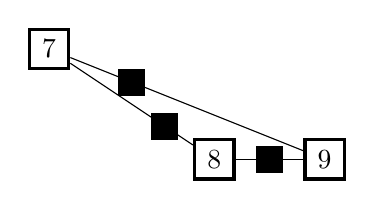
\begin{tikzpicture}[x = 7mm, y=7mm]
%	\draw (-1,-1) rectangle (8,8);
	\tikzstyle{Square} = [
		draw, 
		very thick,
		rectangle,
		minimum size = 5 mm
	]
	\tikzstyle{Synth} = [
		draw, 
		fill = black,
		very thick,
		rectangle,
		minimum size = 3mm
	]
	\tikzstyle{Circle} = [
		draw, 
		circle,
	]
	\tikzstyle{CircleFill} = [
		draw,
		fill = blue, 
		circle,
	]
	\node [Square] (7) at (0,2) {7};
	\node [Square] (8) at (3,0) {8};
	\node [Square] (9) at (5,0) {9};

	\draw (7) -- (8);
	\draw (7) -- (9);
	\draw (8) -- (9);
	
	\node [Synth] () at ($0.3*(7) + 0.7*(8)$) {};
	\node [Synth] () at ($0.7*(7) + 0.3*(9)$) {};
	\node [Synth] () at ($0.5*(8) + 0.5*(9)$) {};


\end{tikzpicture}
\end{center}

One challenge with SMOTE is that it is only useful for datasets with continuous numerical data, and our data is almost all categorical.  What is between ``car'' and ``school bus,'' or between ``parking lot'' and ``highway''?  SMOTE has a variant, SMOTE-NC (Nominal and Continuous) that can handle datasets with some nominal (categorical) features, but most of the features need to be continuous; thus, we will not be able to use SMOTE or similar techniques for our work.  


%%%
\subsubsection{Tomek's Links}

\cite{ivan1976two} proposed a method of undersampling that assumes that the majority and minority classes should (at least locally) be clustered.  If an sample $A$ of the majority class and a sample $B$ of the minority class are each other's nearest neighbors, then one of them is not clustered with its own class.  Since we are trying to undersample the majority class, assume that the element of the majority class is noise (or an error, or just not useful), and delete it.  

In the diagram below, samples \#1 and \#7 are Tomek links, because they are each other's nearest neighbors and of different classes.  Samples \#4 and \#9 are not Tomek links, because while 9 is 4's nearest neighbor, 9's nearest neighbor is 8, not 4.  

In the context of modeling crash severity from police reports, why would sample \#1 not need an ambulance when its characteristics are so close to those of \#7 and not near most of the other crashes without serious injury?  The reason could be errors in the records, or luck/providence/fate.  It could also be that the difference between property damage only and serious injury is influenced by thousands of variables we cannot measure or know, all of the physics of crash forces acting on the bones and structures of the human body.  The best we can say is that the outcome in \#1 cannot be predicted by the information that we have, so that sample will not help in constructing a model based on the available data; therefore, we can reasonably delete it from the training set.  

Tomek's Links can be run repeatedly.  Sample \#7 had \#1 as its nearest neighbor, but once \#1 is deleted, then \#2 and \#7 are each other's nearest neighbors of different classes, thus are Tomek links, and we can delete \#2.  



\begin{center}
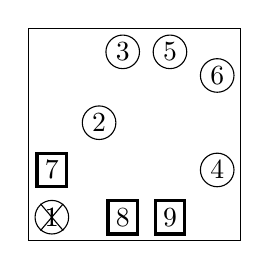
\begin{tikzpicture}[x = 3mm, y=3mm]
	\draw (-1,-1) rectangle (8,8);
	\tikzstyle{Square} = [
		draw, 
		very thick,
		rectangle,
		inner sep = 1mm,
		minimum size = 3 mm
	]
	\tikzstyle{SquareFill} = [
		draw, 
		fill = black,
		very thick,
		rectangle,
	]
	\tikzstyle{Circle} = [
		draw, 
		circle,
		inner sep = 0.5 mm
	]
	\tikzstyle{CircleFill} = [
		draw,
		fill = blue, 
		circle,
	]
	\node [Circle] (1) at (0,0) {1};
	\node [Circle] (2) at (2,4) {2};
	\node [Circle] (3) at (3,7) {3};
	\node [Circle] (4) at (7,2) {4};
	\node [Circle] (5) at (5,7) {5};
	\node [Circle] (6) at (7,6) {6};
	\node [Square] (7) at (0,2) {7};
	\node [Square] (8) at (3,0) {8};
	\node [Square] (9) at (5,0) {9};

	\node [Circle, cross out] (1) at (0,0) {1};
\end{tikzpicture}
\end{center}




%%%
\subsection{Modifying the Loss Function}

Machine learning algorithms generally work iteratively by picking a starting point for the constants in the model (often a random guess), measuring the error, making a small perturbation in the model constants, measuring the new error in the candidate model, and comparing the two.  If the new error is less, use the candidate model; if not, go back to the old one.  Repeat.  

A common way to measure the error in binary classification is log loss (binary cross-entropy loss, logistic loss).  For each sample in the training set we have the answer to the question (the {\it label}), 0 for ``no ambulance,'' 1 for ``ambulance,'' and the candidate model gives a probability $p \in (0,1)$ that this sample will need an ambulance.  The log loss is the sum over the samples of the log of the error.  If the sample is in the majority class, the true value is 0, and if the model gives a value of $p$, then $\log(1-p)$ gives $\log(1)=0$ if the model is perfectly correct and $\log(0) = -\infty$ if the model is perfectly wrong on this sample.  Similarly, for a sample in the minority class, $\log(p)$ gives $\log(1) = 0$ if the model correctly classifies the sample.  If $y$ is the label, then the log loss for each sample is \citep{scikit-learn}

$$L(y,p) = -
	\left( 
		y \log \left( p \right) + \left( 1-y \right) \log \left( 1-p \right) 
	\right) 
$$

Note that if $y=0$, then the first term is 0 for any value of $p$, so only the second term (majority class) is relevant; correspondingly, if $y=1$, then only the first term is relevant, so a clearer expression might be

$$L(y,p) = - 
	\left( 
		\left[ 
			\text{Loss if minority class } (y=1) 
		\right] + 
		\left[
			\text{Loss if majority class } (y=0)
		\right]
	\right) 
$$


 Since the logs of $p \in (0,1)$ will be negative, the negative in front makes the loss positive, and the iterations of the algorithm will seek to minimize it.  

%%%
\subsubsection{Class Weights (Sample Weights, Cost Sensitive Analysis)}

Class weights change the error metric, giving more weight to misclassification of minority class samples \citep{edsjsr.2579163720010401}.  Giving double weight to misclassified minority class samples would have the same effect as duplicating all of the negative class samples in oversampling.  To achieve balance in the contribution of the two classes to the loss function,  

$$\text{Let } r = \frac{ \text{Total number of samples}}{\text{Number of minority samples}} \qquad  \text{Let } \alpha = \frac{r}{r+1} \qquad 1-\alpha = \frac{1}{r+1}$$



$$L(y,p,\alpha) = - 
	\left( 
		\alpha y \log \left( p \right) + 
		\left( 1-\alpha \right) \left( 1-y \right) \log \left( 1-p \right) 
	\right) 
$$


%%%
\subsubsection{Focal Loss}

This method is recent, but has appeared in the crash analysis (see \cite{YU2020102740} referenced below).  Focal loss \citep{lin2017focal} adds another factor to the loss function that gives more weight to samples that are badly misclassified, and less weight to samples that are slightly misclassified.  

$$L(y,p,\alpha, \gamma) = - 
	\left( 
		\alpha y \log \left( p \right)  \left( 1-p \right)^\gamma
		+ 
		\left( 1-\alpha \right) \left( 1-y \right) \log \left(1-p \right) p^\gamma 
	\right) 
$$

The paper by Lin et al. tested values of $\gamma \in [0.0, 5.0]$, and found that $\gamma = 2.0$ gives good balance, but the best value depends on the dataset and the goals.  Yu et al's paper using focal loss for real-time crash prediction allowed the $\gamma$ for minority and majority classes to have different values.  

$$L(y,p,\alpha, \gamma_1, \gamma_2) = - 
	\left( 
		\alpha y \log \left( p \right)  \left( 1-p \right)^{\gamma_1}
		+ 
		\left( 1-\alpha \right) \left( 1-y \right) \log \left(1-p \right) p^{\gamma_2}
	\right) 
$$

%%%
\subsubsection{Comparison of Loss Functions}

The table below compares the three loss functions.  For $\alpha$, we will assume that the minority class is 10\% of the dataset, so 
$r = 10 \to \alpha = r/(r+1)= 10/11 \approx 0.9090$.
For focal loss, we will use $\gamma = 2$.  

Machine learning algorithms use the loss function when comparing two candidate models, only asking which one is less, with no concern for the actual magnitude.  For this reason, the choice of base for the logarithm is inconsequential (we arbitrarily choose base 10 for the chart below); also, that the raw focal loss values are each less than the raw class weights, which are each less than the raw log loss, is not relevant, so we have included normalized values for comparing the three loss functions.  

\begin{center}
\begin{tabular}{ccc|ccc|ccc<{\vrule width 0pt height 12pt depth 4pt}}
	&&& \multicolumn{3}{c}{Raw} & \multicolumn{3}{c}{Normalized} \cr
	Class & y & p & Log & Class & Focal & Log & Class & Focal \cr
	&&& Loss & Weights & Loss & Loss & Weights & Loss \cr\hline
%	Class & y & p & Log Loss & Class Weights & Focal Loss & Log & Class & Focal \cr	
%	& & & $-y \log p$ & $-\alpha y \log p$ & $-\alpha y \log p (1-p)^\gamma$ \cr\hline 
		\multirow{3}{*}{Minority} & 1 & 0.9 & 0.04576 & 0.04160 & 0.00042  & 0.04560 & 0.08292 & 0.00464  \cr
	& 1 & 0.7 & 0.15490 & 0.14082 & 0.01267  & 0.15438 & 0.28069 & 0.14136 \cr
	& 1 & 0.5 & 0.30103 & 0.27366 & 0.06842 & 0.30002 & 0.54548 & 0.76309 \cr\hline
	\multirow{3}{*}{Majority} & 0 & 0.5 & 0.30103 & 0.02737 & 0.00684 & 0.30002 & 0.05455 & 0.07631 \cr
	& 0 & 0.3 & 0.15490 & 0.01408 & 0.00127 & 0.15438 & 0.02807 & 0.01414 \cr
	& 0 & 0.1 & 0.04576 & 0.00416 & 0.00004 & 0.04560 & 0.00829 & 0.00046	 \cr
\end{tabular}
\end{center}

Note that, with focal loss, most of the total loss comes from the one badly misclassified minority sample, so to minimize the loss, the algorithm needs to do a better job classifying that sample.  

%%%
\subsection{Algorithm-Level Methods for Imbalanced Data}



%%%
\subsubsection{Bagging}

``Bagging'' is short for Bootstrapped Aggregating, a variation on random undersampling \citep{BRIEMAN_1996}.  In general, bagging takes many random subsets (with replacement) of the samples, run the classifier on each subset, then aggregate the results.  In imbalanced data applications, each subset of the samples is all of the $n$ minority samples and $n$ randomly chosen majority samples.  

Balanced Random Forest [need citation] is a form of bagging.  

In our example, bagging would make a subset of the data with the three minority-class samples (\#7, 8, and 9), and three randomly chosen from the majority-class samples, run the classifier; repeat some number of times.  Use an ensemble classifier to merge the results.  

\begin{center}
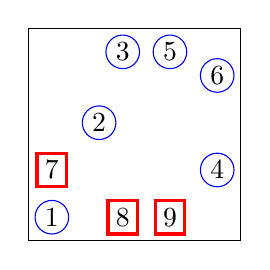
\begin{tikzpicture}[x = 3mm, y=3mm]
	\draw (-1,-1) rectangle (8,8);
	\tikzstyle{Square} = [
		draw = red, 
		very thick,
		rectangle,
		inner sep = 1mm,
		minimum size = 2 mm
	]
	\tikzstyle{SquareFill} = [
		draw = red, 
		fill = red,
		very thick,
		rectangle,
	]
	\tikzstyle{Circle} = [
		draw = blue, 
		circle,		
		inner sep = 0.5mm,
	]
	\tikzstyle{CircleFill} = [
		draw = blue,
		fill = blue, 
		circle,
	]
	\node [Circle] (1) at (0,0) {1};
	\node [Circle] (2) at (2,4) {2};
	\node [Circle] (3) at (3,7) {3};
	\node [Circle] (4) at (7,2) {4};
	\node [Circle] (5) at (5,7) {5};
	\node [Circle] (6) at (7,6) {6};
	\node [Square] (7) at (0,2) {7};
	\node [Square] (8) at (3,0) {8};
	\node [Square] (9) at (5,0) {9};

\end{tikzpicture}
\end{center}


%%%
\subsubsection{Boosting}

Boosting is an iterative method that runs the classifier multiple times.  At the end of each iteration, it determines which samples would be misclassified under the current model.  In the next iteration, the classifier gives higher weight to the misclassified samples, improving the model on marginal cases.  While boosting is not just for imbalanced data, the challenge in imbalanced data is that the minority class samples get misclassified, so boosting would help.  A popular implementation is AdaBoost, introduced by \cite{FREUND1997119}.

%%%%%
\subsection{Using Different Metrics to Evaluate a Model built on Imbalanced Data}

Our goal in building a model is to make an informed guess about a future situation, in our case data from an automated call from the phone of a person involved in a crash.  Does the person need an ambulance?  We don't know for certain, but using past examples we want a model that will make an informed guess.  

To build a model (in supervised learning), we have a set of data (historical data in our case) for which we know the answer to the question, ``Did this crash person need an ambulance?''   We split the data into two parts, training and test, use the training data to build a model, then evaluate the quality of the model using the test data, for which we now have both the actual answer to the question and the model's educated guess.  

When building a model, we test many different models with different algorithms and hyperparameters (user-set parameters, like the $\gamma$ in Focal Loss) and see which model best solves our problem.  To compare two models, we need a metric.

When testing a candidate model, for each sample in the test set, the model returns a probability $Pr \in (0,1)$ that the sample is a member of the positive (minority) class, in our case, the probability that the crash person needs an ambulance.  We then use a threshold ($0.5$ by default) to classify the prediction as negative (N, 0) if the probability is less than the threshold, and positive (P, 1) if more.  Then we compare the prediction with the actual classification (ground truth), which we can organize into a confusion matrix (truth table).  

\begin{center}
\begin{tabular}{cc|c|c|}
	&\multicolumn{1}{c}{}& \multicolumn{2}{c}{Prediction} \cr
	&\multicolumn{1}{c}{} & \multicolumn{1}{c}{N} & \multicolumn{1}{c}{P} \cr\cline{3-4}
	\multirow{2}{*}{Actual}&N & TN & FP \vrule width 0pt height 10pt depth 2pt \cr\cline{3-4}
	&P & FN & TP \vrule width 0pt height 10pt depth 2pt \cr\cline{3-4}
\end{tabular}
\end{center}

The most obvious metric is {\it accuracy}, the proportion of classifications that were successful.  

$$\text{Accuracy} = \frac{ \text{TN} + \text{TP}}{\text{TN} + \text{FP} + \text{FN} + \text{TP}}$$

Because accuracy gives the same weight to the two classes, it may not be the best metric for imbalanced data sets (because it may overfit the majority class), nor for situations where the cost of a false positive (sending an ambulance when one is not needed) is different from the cost of a false negative (not sending an ambulance when one is needed).  Both situations apply to our problem, so we need to consider different metrics, some of which are affected by data imbalance, and some not.

%%%
\subsubsection{Recall}

Recall, or the True Positive Rate (TPR), in our context is, of the calls that actually needed an ambulance, what proportion did the model classify correctly?  
Increasing recall would save lives.  
We really want this number to be high, and are willing to trade off other errors to achieve that goal.  

$$\text{Recall} = \frac{ 
%	\text{TN} 
%	+ 
	\text{TP}
	}{
%	\text{TN} 
%	+ 
%	\text{FP} 
%	+ 
	\text{FN} 
	+ 
	\text{TP}
}$$

Recall only considers the positive (minority) class of the dataset, so it is unaffected by class imbalance.  

%%%
\subsubsection{True Negative Rate}

True Negative Rate (TNR, Selectivity, or Specificity), in our context is, of the calls that did not need an ambulance, what proportion did the model classify correctly?  

$$\text{TNR} = \frac{ 
	\text{TN} 
%	+ 
%	\text{TP}
	}{
	\text{TN} 
	+ 
	\text{FP} 
%	+ 
%	\text{FN} 
%	+ 
%	\text{TP}
}$$

TNR is also not affected by class imbalance because it only considers the classification of the negative (majority) class.  

%%%
\subsubsection{Precision}

Precision in our context is, of the ambulances the model would say to send, what proportion were actually needed?  Increasing precision would save money.  

$$\text{Precision} = \frac{ 
%	\text{TN} 
%	+ 
	\text{TP}
	}{
%	\text{TN} 
%	+ 
	\text{FP} 
%	+ 
%	\text{FN} 
	+ 
	\text{TP}
}$$

Note that precision considers elements of both the majority and minority classes, so class imbalance affects the precision, but we can fix that.  

%%%
\subsubsection{Balanced Accuracy and Balanced Precision}

Balanced accuracy solves the first problem with accuracy, that it is biased towards the majority class.  To balance accuracy, start with the definition of accuracy and scale the majority (negative) class elements (True Negative and False Positive) by the proportions of the positive to negative class, P/N.  The results turns out to be the average of the true positive rate and the true negative rate (derivation in the technical paper).  That TPR and TNR are unaffected by class imbalance confirms that balanced accuracy is unaffected.  

$$	\text{Balanced Accuracy} =  
\frac{ 
	\left(
		\text{TN} \cdot \frac{\text{P}}{\text{N}}
	\right)
	 + \text{TP}
}{
	\left(
		\text{TN} \cdot \frac{\text{P}}{\text{N}}
	\right)
	 + 
	 \left(
	 	\text{FP} \cdot \frac{\text{P}}{\text{N}}
	\right) 
	+ \text{FN} + \text{TP}
}
= \frac{\text{TPR} + \text{TNR}}{2}
$$



In the same way, we can make a balanced precision.  It can also be written in terms of TPR and TNR, (derivation in the technical paper), or more naturally in terms of TPR and the false positive rate (FPR), the proportion of the negative (minority) class that the model misclassified as positive.  In our application, FNR is the proportion of crash persons who did not need an ambulance to whom the model recommends that we should send an ambulance. We have not seen this metric in the literature.  We developed it because balanced accuracy is used extensively in the literature, and it seemed natural to want to balance a useful metric (precision) in the same way that accuracy has been balanced.

$$\text{Balanced Precision} 
= \frac{\text{TP}}{\text{TP} +  \left( \text{FP} \cdot \frac{\text P}{\text N}\right) }
= \frac{\text{TPR} + (1 - \text{TNR})}{\text{TPR}} 
= \frac{\text{TPR} + \text{FPR}}{\text{TPR}} 
$$


%%%
\subsubsection{F1 and G-Mean}

These two popular metrics are each the combination of two other metrics.  

F1 is the harmonic mean of Precision and Recall.  It is often weighted to emphasize one or the other; if $\alpha = 0.5$, the weighted is the same as the original.  We can also substitute Balanced Precision (above) to make a Balanced F1. 

\begin{align*}
	\text{F1} &= \frac{2}{\frac{1}{\text{Precision}} + \frac{1}{\text{Recall}}} 
	= \frac{2 \cdot TP}{2\cdot TP + FP + FN}\cr
	\text{$\alpha$-weighted F1} &= \frac{1}{\frac{\alpha}{\text{Precision}} + \frac{1 - \alpha}{\text{Recall}}} \cr
	\text{Balanced F1} &= \frac{2}{\frac{1}{\text{Balanced Precision}} + \frac{1}{\text{Recall}}} 
\end{align*}


Gmean is the geometric mean of Precision and Specificity (TNR).

$$
	\text{Gmean} = \sqrt{ \text{Precision} \times \text{Specificity}} 
	= \sqrt{
		\frac{TP}{TP+FP} \times \frac{TN}{TN+FP}
		}
$$

In this paper we have a binary classification model, but
\cite{LIU2021103070} adapted class-weighted F1 for classification of multiple classes in a multi-modal recommendation system.  That paper has an excellent discussion of why and how they applied the class-weighted F1 metric in post-processing, because the metric is not differentiable.  

%%%
\subsubsection{Over-Predicting the Minority Class [Needs Citations]}

One tests a model by using it to classify the samples in a test subset of the data.  For each sample, the model gives a probability $Pr \in (0,1)$ that the sample belongs to the positive class.    Ideally, most of the samples will fall close to the extremes, clearly classified as either positive or negative, indicating that our model is strong and is more likely to correctly classify future samples, but in practice many samples will not be so clearly classified.  

The bar graph below illustrates one model classifying the samples of the CRSS dataset into negative (red, ambulance not needed, majority class) and positive (blue, ambulance needed, minority class).  The horizontal axes represents the probability $Pr \in (0,1)$ given by the model that a sample belongs to the class, and the vertical is the number of samples that fall in each probability range.  

\begin{center}
	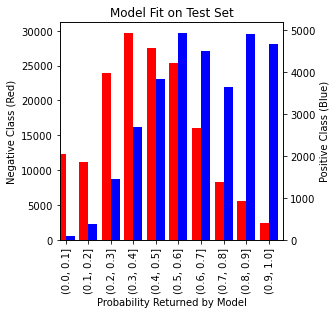
\includegraphics[scale=0.8]{Model_Probabilities_by_Class.png}
\end{center}

By default, one uses a threshold $Pr = 0.5$ to assign the samples to the negative (majority, $Pr < 0.5$) or positive (minority, $Pr > 0.5$) classes, but we are free to change that threshold.  In the bar graph, all red elements to the left of the threshold are TN, all red elements to the right are FP, all blue elements to the left are FN, and all blue elements to the right are TP.  The threshold is a hyperparameter that affects all of the above metrics; for example, decreasing the threshold would shift samples from TN to FP, and from FN to TP.   Decreasing the threshold would over-predict the minority class, and increasing it would under-predict.  

The chart below gives metrics on that model on the CRSS dataset for different thresholds $t$.  The last column is the marginal tradeoff between unneeded ambulances sent and needed ambulances not sent; for instance, at threshold $p = 0.50$, the difference between $p = 0.45$ and $p = 0.55$ is 5.99 ambulances unnecessarily sent for every needed ambulance not sent.  If we (as a society) believe that that cost is too high and we should send fewer ambulances, we should choose a larger threshold value and under-predict the minority class.  For the purposes of this paper we have arbitrarily chosen 10 as the number of additional false alarms we are willing to tolerate for each additional ambulance sent when needed, so we could change the threshold to somewhere in $0.3 < t < 0.4$, over-predicting the minority class.

% From CRSS_07_01_22_ROC_Curves
\begin{center}
\begin{tabular}{r*8{|r}}
	\multicolumn{1}{c|}{$t$}  & \multicolumn{1}{c|}{TN} & \multicolumn{1}{c|}{FP} & \multicolumn{1}{c|}{FN} & \multicolumn{1}{c|}{TP} & \multicolumn{1}{c|}{TPR} & \multicolumn{1}{c|}{FPR} & 
	$\displaystyle \frac{ \Delta \text{TPR}}{\Delta \text{FPR}}$ &
	$\displaystyle \frac{ \Delta \text{FP}}{\Delta \text{TP}}$ \vrule width 0pt depth 12pt \cr\hline
	0.00 & 0 & 162200 & 0 & 31083 & 1.00 & 1.00 & 0.02 & 246.76 \cr
0.10 & 12322 & 149878 & 84 & 30999 & 1.00 & 0.92 & 0.09 & 58.08 \cr
0.20 & 23556 & 138644 & 455 & 30628 & 0.99 & 0.85 & 0.26 & 20.33 \cr
0.30 & 47541 & 114659 & 1895 & 29188 & 0.94 & 0.71 & 0.37 & 14.10 \cr
0.40 & 77254 & 84946 & 4590 & 26493 & 0.85 & 0.52 & 0.60 & 8.74 \cr
0.50 & 104764 & 57436 & 8425 & 22658 & 0.73 & 0.35 & 0.87 & 5.99 \cr
0.60 & 130098 & 32102 & 13362 & 17721 & 0.57 & 0.20 & 1.23 & 4.25 \cr
0.70 & 146094 & 16106 & 17860 & 13223 & 0.43 & 0.10 & 1.77 & 2.95 \cr
0.80 & 154351 & 7849 & 21506 & 9577 & 0.31 & 0.05 & 3.09 & 1.69 \cr
0.90 & 159855 & 2345 & 26404 & 4679 & 0.15 & 0.01 & 8.00 & 0.65 \cr
1.00 & 162200 & 0 & 31083 & 0 & 0.00 & 0.00 & 14.18 & 0.37 \cr

\end{tabular}
\end{center}

%%%
\subsubsection{Area Under the ROC Curve [Needs Citations]}

The Receiver Operating Characteristic (ROC) shows how much the positive and negative classes are interleaved.  It is a parameterized curve following the probability threshold from $t=0$ to $t=1$, and plotting the true positive rate (TPR) versus the false positive rate (FPR).  The orange ``Model''  curve in the graph below is from the same dataset predictions in the chart above.  The eleven points correspond to the (FPR,TPR) coordinates in the chart, going from $t=0.0$ in the upper right to $t=1.0$ in the lower left.    The next-to-last column in the chart gives the slope of the ROC curve.  

If the model gave entirely random results, the bars in the bar chart above would all have the same height (1/20 of the number of elements in the class), and the slope of the ROC curve would be 1, illustrated by the green line, and the area under the curve (AUC) would be $0.5$.  If our model and dataset were ideal, with all of the negative elements having $Pr=0.0$ and all of the positive elements having $Pr=1.0$, the ROC curve would be the blue $\Gamma$, with area under the curve of 1.0.  In practice, the area under the curve is between 0.5 and 1.0.  

The area under the ROC curve is useful for comparing different models on the same dataset.  A higher area generally means that the model more clearly separates the two classes, and is more likely to correctly classify elements of a different (but related) set of samples.

Because both TPR and FPR are unaffected by class imbalance, the ROC curve is as well.  



\begin{center}
	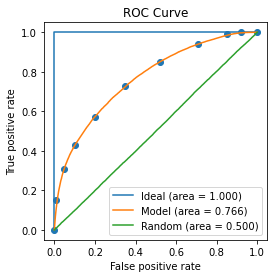
\includegraphics[scale=0.8]{ROC_Example.png}
\end{center}

%%%%% Lit Review






%\cite{7727770} Wang, Training deep neural networks on imbalanced data sets, cited in Formosa 2020 with ``Deep Neural Network (DNN) models with a Mean Squared False Error loss function have the ability to capture classification errors from both majority and minority classes equally (Wang et al., 2016)''

%\cite{PENG2020105610} used cost-sensitive MLP algorithm, which was developed by \cite{6469237}.  MLP is Multi-Layer Perceptron.


%%%
\subsection{Imbalanced Data in Crash Analysis}

Imbalanced data is a frequent concern in crash analysis.  In crash prediction, ``non-crash'' samples are much more numerous than ``crash'' samples. 

%%%
\subsubsection{Oversampling}

%
\cite{PARSA2019202} used SMOTE to balance the dataset of crashes on Chicago's Eisenhower expressway.  
%
\cite{LI2020105371} used SMOTE to study crashes on urban arterials.  
%
\cite{GUO2021106328} used SMOTE to consider risky driving behavior in crash prediction.  
%
\cite{ORSINI2021106382} used SMOTE in building a a real-time conflict prediction model.
%
\cite{ELAMRANIABOUELASSAD2020102708} used SMOTE in studying crash prediction for collision avoidance systems.  
%
\cite{MORRIS2021106240} compared three oversampling methods, 
random over-sampling, SMOTE, and adaptive synthetic sampling, for crash data analysis.  
%
\cite{YAHAYA2021105936} compared three oversampling methods studying contributing factors in fatal crashes in Ghana, and the same group applied the majority weighted minority oversampling (MWMOTE) method to study multiple fatal injury crashes \citep{YAHAYA2021105851}.


%%%
\subsubsection{Multiple Techniques}
%
\cite{SCHLOGL2019134} used SMOTE and maximum dissimilarity undersampling to balance an Australian dataset to build a model to predict crashes, while in a later paper Sch\"{o}gl used a balanced bagging approach \citep{SCHLOGL2020105398}.    
%
\cite{CHEN2020102646} used SMOTE and Tomek's links in studying crash potential in lane-changing behavior.  
%
\cite{PENG2020105610} used undersampling, SMOTE, cost-sensitive algorithms, and boosting.  
%
\cite{LI2021106422} used the proximity weighted synthetic oversampling technique (ProWSyn) method to build a traffic violation prediction model.
%
\cite{CHEN2022106496} compared Synthetic Minority Over-Sampling Technique for panel data (SMOTE-P) with Random Under-sampling of the Majority Class (RUMC) technique, Cluster-Based Under-Sampling (CBUS), and mixed resampling to identify explanatory factors that affect the crash risk of buses in Hong Kong.
%
\cite{CHEN2020102646} used ENN-SMOTE-Tomek Link (EST) in estimating crash risk in lane changing.  



%%%
\subsubsection{Image (or Image-like) Data}
%
\cite{FORMOSA2020105429} used Deep Neural Network (DNN) models with a Mean Squared False Error loss function to analyze images from front-facing cameras in cars on a UK roadway to predict crashes.  
%
% Not images?
\cite{LIN2020105628} used Generative Adversarial Networks (GAN) to overcome data imbalance for their incident detection model.  
%
\cite{ISLAM2021105950} found that a variational autoencoder was more useful than SMOTE, ADASYN, and GAN for generating minority samples to balance crash and non-crash events.  
%
\cite{BASSO2021106409} used Deep Convolutional Generative Adversarial Networks technique with random undersampling to use image and image-like data to build an accident-prediction model for a section of highway in Chile.  
%
\cite{MAN2022106511} used Wasserstein GAN (WGAN) and random undersampling to study the transferability of a model built on one dataset to other datasets.  
%
\cite{CAI2020102697} compared deep convolutional generative adversarial network (DCGAN) with SMOTE and random undersampling to study the effects of proactive traffic safety management strategies such as variable speed limits and dynamic message signs.  

%%%
\subsubsection{Other}
%
\cite{LACK2021106105} used bagging in predicting crashes for trucks and finding ways to improve truck safety.  
%
\cite{HAULE2021106181} used boosting in studying the effects of ramp metering on traffic safety.  
%
\cite{YU2020102740} implemented the new focal loss technique in real-time crash prediction.
%
\cite{SHI2019170} used undersampling to analyze factors predicting risky and safe driving.  
%
\cite{ZHU2021106199} used cost-sensitive semi-supervised logistic regression (CS3LR) for hit-and-run analysis.  



%%%
\subsubsection{Imbalanced Data in Other Transportation Areas}

%
\cite{MOHAMMADI2019153} used 
the Adaptive Synthetic Sampling Approach (ADASYN) on a dataset of foot-by-foot track geometry and tonnage to identify the factors that predict rail defects.
%
\cite{SHI2021103414} developed a
hierarchical over-sampling bagging method based on Grey Wolf Optimizer (GWO) algorithm and Synthetic Minority Over-sampling Technique (SMOTE)
to study lane changing for autonomous vehicles.  The data was severely imbalanced because lane changing is rare compared with lane keeping.
%
\cite{KHAN2021103225} used SMOTE and Tomek links and ``average balanced recall accuracies'' for flight delay prediction.  
%
\cite{CHEN2022103709} used bagging for ride-hailing demand prediction.  
 
%%%
%
% Needs work
%
%%%

In crash severity, most reported crashes are just property damage only (PDO), and many PDO crashes aren't even reported.  Other aspects of transportation also have imbalanced data, including 

\begin{itemize}
	\item \cite{JIANG2020105520} used similar data and addressed the challenges we'll have with it.  
	\item \cite{ELAMRANIABOUELASSAD2020102708} works with several imbalanced methods.  Use this paper as a model.  
\end{itemize}

%%%
\subsubsection{Ambulances}

\begin{itemize}
	\item \cite{PARK2019230} has a full-page table categorizing studies of ambulance location, relocation, and dispatching using different optimization methods.  
\end{itemize}



%%%%% Datasets
%%%%%
\section{Datasets}

The dataset we want for this study, unfortunately, does not exist.  Such a dataset would have several years of automatic notifications from cell phones to police of a crash, with accompanying data on (a) whether it actually was a crash, (b) whether the user of that phone needed an ambulance, and (c) whether anyone else involved in the crash needed an ambulance.  The dataset does not yet exist because the technology is too new.  The app developers must have testing data, but we have not seen any publicly available.  

To do the best work we can with what is available, we need an appropriate proxy dataset, but that will be challenging.  We do not know how well the apps detect a crash, currently or in the future.  For instance, if the crashes the apps detect were those crashes where the airbag deploys, they would miss most of the crashes requiring an ambulance.  (These data are from CRSS; see below.)  

\begin{center}
\begin{tabular}{cr|r|r|}
	&\multicolumn{1}{c}{}& \multicolumn{2}{c}{Air Bag Deployed} \cr
	&\multicolumn{1}{c}{} & \multicolumn{1}{c}{No} & \multicolumn{1}{c}{Yes} \cr\cline{3-4}
	\multirow{2}{*}{Ambulance}& No & 479,287 & 61,377 \vrule width 0pt height 10pt depth 2pt \cr\cline{3-4}
	& Yes & 64,699 & 38,911 \vrule width 0pt height 10pt depth 2pt \cr\cline{3-4}
\end{tabular}
\end{center}

The apps using the phone's accelerometer will have a hard time distinguishing low-speed crashes from hard braking, so the apps will not detect many non-injury crashes; therefore, we may need to either underrepresent non-injury crashes in our work, or start with a database that does that, like CRSS.  

For this study we used two datasets, the Crash Report Sampling System 2016-2020 \citep{CRSS}, and a tabular assembly of all of the Louisiana crash records 2014-2018.  While the CRSS data and a helpful guide are available online, the Louisiana data is not publicly available.  

%%%
\subsection{CRSS:  Crash Report Sampling System}

CRSS, as its name suggests, is a curated sample of crashes in the US, scrubbed of personally identifying information and with missing values imputed. It is intentionally not a representative sample, but intentionally over represents serious crashes; for instance, ``crashes with killed or injured pedestrian'' represent 9\% of the crashes in the dataset but only 1.9\% of crashes in the US.   Its sample design is given on page 18 of the CRSS Analytical Users Manual \citep{CRSS_Manual}.  Because the dataset is not representative, we have to be careful in drawing inferences.  Since we do not know, in detail, the present and future capabilities of the cell phone app, this dataset that overrepresents more serious crashes may be a good proxy, and we will use it as such.    


%%%
\subsection{Louisiana Data}

The structure of the Louisiana data is similar to CRSS.  Key differences are that it is a census of all crash reports, and missing data is not imputed.   While CRSS data is given entirely in attribute codes, many fields in the Louisiana data, like city and street names, are text, uncorrected; the city of Shreveport is spelled at least nineteen different ways.  


%%%%%
\subsection{Imputing Missing Data}

All data is dirty, with incorrect and missing values.  The CRSS dataset is reasonably correct in that only the values that should appear in a feature actually appear; for instance, a feature that should have numerical values does not have text values for a few samples.  For CRSS, we will not tackle the question of whether the values are correct, but most of the features have values that signify ``Missing'' or ``Unknown,'' and we want to impute values for those incomplete samples, using data in other features. 

The methods for imputing those values are well developed.  If the feature were continuous numeric, we could use the Numpy, Pandas, and scikit-learn methods to replace missing values in a feature with the mean or median of that feature.  For categorical data, the same packages will impute the most common value in that feature.    

In CRSS, the data is almost all categorical, and the data is so imbalanced that the most common value often corresponds to a minor crash with no injury.  To impute values using the most common value in the feature would make our dataset even more imbalanced.  For instance, of the 644,274 people in the dataset, 429,574 (67\%) of the people have ``No Apparent Injury,'' and 21,595 (3.3\%) are ``Unknown/Not Reported.''  Assigning the most common value in that feature to the missing elements would worsen the imbalance; a better method would build a model of the data and use the model to fill in the holes.  

Scikit-learn does have an experimental multiple imputation method, but it only works for continuous data.  

The CRSS authors used a Sequential Regression Multivariate Imputation (SRMI) method to impute missing data in some features, employing the implementation in the University of Michigan's ``IVEware:  Imputation and Variance Estimation Software''  \citep{IVEware}.  

In \verb|SEX|, for instance, the samples attributes ``Not Reported'' and ``Reported as Unknown'' are assigned to either ``Male'' or ``Female'' in the feature \verb|SEX_IM|.

\begin{center}
\begin{tabular}{cr|r|r|}
	&\multicolumn{1}{c}{}& \multicolumn{2}{c}{Imputed} \cr
	&\multicolumn{1}{c}{} & \multicolumn{1}{c}{Male} & \multicolumn{1}{c}{Female} \cr\cline{3-4}
	\multirow{4}{*}{Original}& Male & 339,365 & 0 \vrule width 0pt height 10pt depth 2pt \cr\cline{3-4}
	&Female & 0 & 278,766 \vrule width 0pt height 10pt depth 2pt \cr\cline{3-4}
	& Not Reported & 8,748 & 7,168 \vrule width 0pt height 10pt depth 2pt \cr\cline{3-4}
	& Reported as Unknown & 5,799 & 4,428 \vrule width 0pt height 10pt depth 2pt \cr\cline{3-4}
\end{tabular}
\end{center}

The CRSS authors did not impute missing values for all of the features, including some we want to use.  The reasons they gave for not imputing more features include wanting to be consistent with the features and methods in the predecessor to CRSS, the National Automotive Sampling System General Estimates System (NASS GES), 1998-2015, which also used IVEware's SRMI in 2011-2015
\citep{CRSS_Imputation}.  Which features are imputed even changes from year to year, for instance with \verb|RELJCT1_IM| being discontinued in 2019 and brought back in 2020.  
Wanting all of the features we were to use to have missing values imputed, we followed CRSS's methods to run IVEware ourselves on the data, using the features imputed by CRSS to check that our process was similar to theirs.  

The table below gives the frequency of values in the \verb|INJ_SEV| feature.  The original values include ``9:  Unknown/Not Reported.''  The last two rows show the results from the CRSS authors' imputations, and our imputations trying to replicate their method.  

\begin{tabular}{llrrrrrrr}
\toprule
INJ\_SEV Imputed &&       0 &      1 &      2 &      3 &     4 &     5 &   6 \\
INJ\_SEV Original &&         &        &        &        &       &       &     \\
\midrule
No Apparent Injury  & 0       &  429574 &      0 &      0 &      0 &     0 &     0 &   0 \\
Possible Injury & 1       &       0 &  95761 &      0 &      0 &     0 &     0 &   0 \\
Suspected Minor Injury & 2       &       0 &      0 &  57299 &      0 &     0 &     0 &   0 \\
Suspected Serious Injury & 3       &       0 &      0 &      0 &  32556 &     0 &     0 &   0 \\
Fatal Injury & 4       &       0 &      0 &      0 &      0 &  5587 &     0 &   0 \\
Injured, Severity Unknown & 5       &       0 &      0 &      0 &      0 &     0 &  1883 &   0 \\
Died Prior to Crash & 6       &       0 &      0 &      0 &      0 &     0 &     0 &  19 \\
Unknown/Not Reported & 9       &   14986 &   4065 &   1401 &    876 &   114 &   153 &   0 \\
Unknown/Not Reported & 9       &   15423 &   3104 &   1777 &   1061 &   180 &    49 &   1 \\
\bottomrule
\end{tabular}



Imputation methods are given on page 19 of the CRSS Analytical User's Manual and in the CRSS Imputation report.  The imputation report gives the model selection criteria used in IVEware, and we have used those in our work, particularly 10 cycles, the minimum marginal r-squared required for a predictor to be included in the model set to 0.01, and the maximum number of predictors in a model set to 15 (footnotes on pages 7 and 8).  

Two feature's imputations are inexplicably different from the others, \verb|MAX_SEV|, the maximum injury severity in a crash, and \verb|NUM_INJ|, the number of people injured in the crash.  Not only are missing values imputed, but some other values are changed.  Another odd imputation is \verb|VEVENT_IM|, the imputed values of \verb|M_HARM|, the most harmful event.  Category 4, ``Gas Inhalation,'' does not appear any of the original samples, but three of the missing entries get imputed to that category.  Perhaps these samples were imputed by hand.  



\begin{center}
\begin{tabular}{cr*9{r|}}
	\multicolumn{1}{c}{} &\multicolumn{1}{c}{} & \multicolumn{1}{c}{} & \multicolumn{8}{c}{Imputed} \cr
	&\multicolumn{1}{c}{Original} 
		& \multicolumn{1}{c}{} 
		& \multicolumn{1}{c}{0} 
		& \multicolumn{1}{c}{1} 
		& \multicolumn{1}{c}{2} 
		& \multicolumn{1}{c}{3} 
		& \multicolumn{1}{c}{4} 
		& \multicolumn{1}{c}{5} 
		& \multicolumn{1}{c}{6} 
		& \multicolumn{1}{c}{8} 
		\cr\cline{2-2}\cline{4-11}
%	\multirow{4}{*}{Original} 
& No Apparent Injury & 0    &      120,142  & 1,300 &   422 &  266  &  29  &  51 &  0  & 0 
	 \vrule width 0pt height 10pt depth 2pt \cr\cline{4-11}
	& Possible Injury & 1 &  0 & 58,392 &   222 &   125  &  16 &    0 &  0 &  0
	 \vrule width 0pt height 10pt depth 2pt \cr\cline{4-11}
	 & Suspected Minor Injury
		 & 2 &   0  &    0 &  40,247  &   93  &  20 &    0 &  0 &  0
	 \vrule width 0pt height 10pt depth 2pt \cr\cline{4-11}
	 & Suspected Serious Injury & 
              3 & 0  &    0  &    0 & 26,767  &   9 &    0 &  0 &  0
	 \vrule width 0pt height 10pt depth 2pt \cr\cline{4-11}
	& Fatal & 
	4   &            0  &    0 &     0  &    0 & 5,115  &   0 &  0 &  0
	 \vrule width 0pt height 10pt depth 2pt \cr\cline{4-11}
	 & Injured, Severity Unknown 
	& 5  &             0  &   16  &    6  &    2  &   1 & 1,250  & 0 &  0
	 \vrule width 0pt height 10pt depth 2pt \cr\cline{4-11}
	 & Died Prior to Crash
	& 6       &        0  &    0  &    0   &   0  &   0   &  0 & 11  & 0
	 \vrule width 0pt height 10pt depth 2pt \cr\cline{4-11}
	& No Person Involved in Crash 	 
	& 8    &           0  &    0  &    0  &    0  &   0  &   0 &  0 & 95
	 \vrule width 0pt height 10pt depth 2pt \cr\cline{4-11}
	 & Unknown/Not Reported 
	& 9      &      2,859  &  887   & 383 &   290 &   38  &  23 &  0 &  0
	 \vrule width 0pt height 10pt depth 2pt \cr\cline{4-11}
\end{tabular}
\end{center}

We considered using \verb|MAX_SEV| as our target variable, but ended up not using it at all.  We instead decided to use \verb|HOSPITAL|, which ``identifies the mode of transportation to a hospital or medical facility provided for this person.''  Five of the values of that data element correspond to the person being transported to a hospital by some means, and the other four either not transported or unknown.  We binned it as in this chart.  

\begin{center}
\verb|HOSPITAL| Field in CRSS

\

\begin{tabular}{c| l  r|r<{\vrule width 0pt height 10pt depth 2pt}}
	\multicolumn{1}{c|}{Binned} & \multicolumn{2}{c|}{Original} & \multicolumn{1}{c}{Count} \cr\hline
	\multirow{4}{*}{FALSE} 
	& Not Transported & 0 & 522,801 \cr
	& Other & 6 & 4,341 \cr
	& Not Reported & 8 & 12,447 \cr
	& Unknown & 9 & 1,075 \cr\hline
	\multirow{5}{*}{TRUE}
	& EMS Air & 1 & 2,549 \cr
	& Law Enforcement & 2 & 605 \cr
	& EMS Unknown Mode & 3 & 30,368 \cr
	& Transported Unknown Source & 4 & 8,926 \cr
	& EMS Ground & 5 & 61,162 \cr	
\end{tabular}
\end{center}

%%%
\subsection{Lit Review:  Imputing Missing Data in CRSS [Rough]}

\begin{itemize}
	\item \cite{TOPUZ2021113557} does a thorough description of imputing missing data in CRSS.  Does not mention IVEware.  Also deals with imbalanced data well.  Need to spend time with this article. 

	\item \cite{COX2021288} says CRSS ``can be
weighted to produce annual national estimates.''  Also, ``Police-reported
crash sampling methods changed when NHTSA converted from
NASS GES to CRSS, which may have affected the comparability of
the 2017 data on all crash involvements with earlier years.''
	
	In this study, 
	``Imputed data were utilized when available to account for missing data.''
	
	\item \cite{AMINI2022108720} gives a thorough description of CRSS.  They took out CRSS-imputed variables.  Also removed post-accident information, as it was not relevant.  They imputed missing continuous variables, but don't say how.  They left missing categorical variables as ``Unknown'' and ``Missing'' categories.  
	
\begin{quote}
	Employing descriptive analytics, we distinguished and removed
variables with a large percentage of missing values (more than 70\%), as
well as the identification, irrelevant, repetitive, and CRSS-imputed
variables. We also removed the variables with post-accident information,
such as whether the vehicle was towed afterward or the number of
injured people. Using such variables contradicts the basic assumption of
time order in causal relations, where a cause should precede its effect.
Furthermore, we handled other missing values by considering them
separate categories for nominal variables and imputing numeric ones.
\end{quote}	

	\item \cite{SPICER2021105974} used CRSS but did not mention missing or imputed data.  
	
	\item \cite{VILLAVICENCIO2022757} says that ``CRSS is a representative
sample of all police-reported crashes in the United States,'' which is not true.  They used FARS and CRSS as their primary data sources, but did not mention imputed or missing data.  
	
	``Each record in CRSS includes a statistical weight to
indicate the number of crashes in the population represented by
each record in the sample.''  
	
	\item \cite{MUELLER2022305} says that ``CRSS sampling weights were used in those data to generate national estimates,'' and ``The CRSS data set handles missing data for some variables by statistically imputing values, which were used when available.''
	
	\item \cite{KAPLAN2017130} uses the phrase, ``restricted access database.''  I should use that for the Louisiana crash database.  
	
	\item \cite{GONG2022100190} just dropped samples with missing values.  
	
	\item As far back as 2002, NHTSA was working on multiple imputation methods for its related database, FARS.  \citep{subramanian2002transitioning}
		
\end{itemize}


%%%%% Methods
%%%%%
\section{Methods}

We used the Crash Report Sampling System (CRSS) \cite{CRSS} data to train and test our model.  After preparing the data, we built a variety of models with different combinations of techniques for handling imbalanced data, model types, loss functions, and sets of features, with the overall goal of finding an optimal combination of methods to give the most useful model.


%%%
\subsection{Feature Selection}

In selecting features from the CRSS dataset, we chose features that could be known or inferred at the time of the crash without an eyewitness.  We separated them into three sets in terms of how hard the data would be to get in good quality:  Easy, medium, and hard.  The easy information is a baseline, the information the police have before they receive the notification, like locality, time of day, and weather.    The medium level requires detailed maps to distinguish between, for example, an intersection and a parking lot, and information from the phone service provider about the primary user of the phone.  The hard level would require coordination of private (cell service providers, Apple Google) and public databases (police, government vehicle registries), or correlating several notifications from different phones at about the same time from about the same location to see that they are probably the same crash event.  


\begin{description}
	\item [Location] \
		 \begin{description}
			\item [Easy]
			\item Region (4 regions of the US)
			\item Principal Sampling Unit (74 subregions of the US)
			\item Police Jurisdiction (422 jurisdictions)
			\item Urban/Rural
		\item [Medium:  Requires precise location and maps]
		 	\item Interstate
			\item In intersection (Yes/No)
			\item Type of interesection
			\item Position relative to the road
			\item Position relative to an intersection
			\item Roadway alignment (curve, straight, driveway,...)
			\item Number of lanes in roadway
			\item Roadway grade
			\item Speed limit
			\item Traffic control device (stop lights, stop signs)
			\item Trafficway description (two way, divided, ramp,...)
			\item [Medium:  Requires up-to-date maps]
			\item Work Zone
		\item [Hard:  Requires very detailed maps]
			\item Relation to junction features
		 \end{description}
	\item [Time] \
		 \begin{description}
	 	\item [Easy]
			\item Hour
			\item Weekday/Weekend
			\item Month
			\item Year
			\item Weather
		\item [Medium:  Requires detailed maps per time of day]
		 	\item Lighting Conditions
		 \end{description}
	\item [Phone User] \
		 \begin{description}
	 	\item [Medium: Requires identifying phone user]
		 	\item Age
			\item Sex
		\item [Medium:  Requires storing acceleration data for several minutes]
			\item Pedestrian / In moving vehicle
		\item [Hard:  Requires identifying the vehicle used by phone user]
			\item Make of vehicle
			\item Model of vehicle
			\item Age of vehicle
			\item Body type of vehicle
		\item [Hard:  Requires identify licensing of phone user (driver) or ages from several phones (bus passengers)]
			\item School bus
			\item Type of other bus
			\item Emergency vehicle
		 \end{description}
	\item [Correlate Multiple Notifications] \ 
		\begin{description}
		\item [Hard]
			\item Number of people in vehicles
%			\item Number of pedestrians
			\item Number of occupants of particular vehicle
			\item Number of vehicles in motion
			\item Number of parked vehicles	
		\end{description}
\end{description}



%%%%%
\subsection{Missing Data}

The CRSS \verb|HOSPITAL| feature, which we used as our target feature, has missing values.  CRSS has imputed missing values for several features, but not for \verb|HOSPITAL|.  

For its imputed features, CRSS used IVEware, which uses sequential regression multivariate imputation (SRMI).  

We first tried to use scikit-learn's SimpleImputer, which imputed all of the missing values as ``0: Not Transported.''

Then we tried scikit-learn's IterativeImputer, but it only works with numerical continuous data, and all of our features are unordered categorical.


%%%
\subsection{Feature Binning}

Above we illustrated how the \verb|HOSPITAL| field had nine attributes, but we put them into two bins.  We were interested only in whether a crash person was transported to a hospital, not exactly how, so for our purposes, ``EMS Air'' and "EMS Ground'' were equivalent.  Several of the features had about ten attributes that we could assign to fewer bins in obvious ways.  Details in the technical paper.

Some features had attributes that did not fall into bins in obvious ways.  Is a ``Compact Pickup,'' a designation that only existed in 2016, more like a sedan or a light pickup?  To draw the lines, we looked at how that attribute correlated with \verb|HOSPITAL|.  The rate at which crash persons in compact pickups were transported to the hospital was (statistically) indistinguishable from sedans (15\%), but very different from light pickups (11\%).  

For \verb|AGE_IM|, age with missing values imputed, we had values 0-120 that we wanted to assign to bins.  The obvious way would have been to do it by decade, but when we looked at the hospitalization rates, patterns emerged.  

In most states in the US, teens can get a driver's license at age 16, but in most states they can get a learner's permit earlier, so in the chart below, some of the 14 and 15 year olds may be the driver.  

In the chart, we see a big shift between 14 and 16, both in the number of crash people and the hospitalization rate.  There is also a big shift between 18 and 21 in hospitalization rate.  Where exactly to draw the line is open for debate, but we made 16-18 a separate group.  The next big shift was in the 50's, and we made 19-52 the next group.  

\begin{center}
\begin{tabular}{lll}
	\multicolumn{2}{l}{Age} \cr
	& \multicolumn{2}{l}{Percent of Total Crash Persons} \cr
	&& Hospitalization Rate (\%) \cr\hline
	 10 & 0.53 & 16.58 \vrule width 0pt height 10pt\cr
	 11 & 0.51 & 15.51 \cr
	 12 & 0.52 & 16.54 \cr
	 13 & 0.54 & 16.72 \cr
	 14 & 0.63 & 17.56 \cr
	 15 & 0.88 & 15.21 \cr
	 16 & 1.65 & 13.46 \cr
	 17 & 2.18 & 14.25 \cr
	 18 & 2.65 & 14.41 \cr
	 19 & 2.67 & 15.47 \cr
	 20 & 2.58 & 14.91 \cr
	 21 & 2.51 & 15.65 \cr
	 22 & 2.56 & 15.43 \cr
	 23 & 2.44 & 15.57 \cr
	 24 & 2.38 & 16.01 \cr
	 25 & 2.37 & 15.50 \cr
\end{tabular}
\end{center}

Full chart in the technical paper.  



%%%
\subsection{Feature Engineering}

From the features in the dataset, we can create new features that may be relevant, like ``Rush Hour,'' combining hour with day of week.  During rush hour, the number of crashes increases, but their average severity goes down.  We drew the lines distinguishing ``Rush Hour'' from "Not Rush Hour'' based, again, on the correlation to hospitalization.  Interestingly, the hospitalization rates varied by age, and varied by sex, but varied differently by age within sex.  Hospitalization rates for young children are low, perhaps due to child seat requirements, but after young childhood, as age increases, the hospitalization rate increases for both men and women, but younger women have a lower hospitalization rate than men, and older women have a higher rate.  We created an \verb|AGE_SEX| feature.  


\begin{center}

\begin{tabular}{lrrr}
\multicolumn{4}{c}{Crash Person Count} \cr
\toprule
{Age} &  Female &    Male &   Total \\
\midrule
00-06 &   12331 &   12639 &   24970 \\
07-15 &   16623 &   16726 &   33349 \\
16-18 &   20158 &   21622 &   41780 \\
19-52 &  175528 &  219931 &  395459 \\
53-70 &   49750 &   65228 &  114978 \\
71+   &   15972 &   17766 &   33738 \\ \hline
Total &  290362 &  353912 &  644274\vrule width 0pt height 10pt \\
\bottomrule
\end{tabular}
\end{center}

\begin{center}
\begin{tabular}{lrrr}
\multicolumn{4}{c}{Hospitalization Count} \cr
\toprule
{Age} &  Female &   Male &   Total \\
\midrule
00-06 &    1448 &   1560 &    3008 \\
07-15 &    2529 &   2779 &    5308 \\
16-18 &    2900 &   2998 &    5898 \\
19-52 &   28843 &  33514 &   62357 \\
53-70 &    9302 &  10947 &   20249 \\
71+   &    3503 &   3287 &    6790 \\ \hline
Total &   48525 &  55085 &  103610\vrule width 0pt height 10pt \\
\bottomrule
\end{tabular}
\end{center}

\begin{center}
\begin{tabular}{lrrr}
\multicolumn{4}{c}{Hospitalization Rate} \cr
\toprule
{Age} &  Female &   Male &  Total \\
\midrule
00-06 &   0.117 &  0.123 &  0.240 \\
07-15 &   0.152 &  0.166 &  0.318 \\
16-18 &   0.144 &  0.139 &  0.283 \\
19-52 &   0.164 &  0.152 &  0.316 \\
53-70 &   0.187 &  0.168 &  0.355 \\
71+   &   0.219 &  0.185 &  0.404 \\ \hline
Total &   0.983 &  0.933 &  1.916\vrule width 0pt height 10pt \\
\bottomrule
\end{tabular}
\end{center}

\begin{center}
\begin{tabular}{lrrr}
\multicolumn{4}{c}{Rate Normalized by Row} \cr
\toprule
{Age} &  Female &   Male &  Total \\
\midrule
00-06 &   0.488 &  0.512 &    1.0 \\
07-15 &   0.478 &  0.522 &    1.0 \\
16-18 &   0.509 &  0.491 &    1.0 \\
19-52 &   0.519 &  0.481 &    1.0 \\
53-70 &   0.527 &  0.473 &    1.0 \\
71+   &   0.542 &  0.458 &    1.0 \\ \hline
Total &   3.063 &  2.937 &    6.0\vrule width 0pt height 10pt \\
\bottomrule
\end{tabular}
\end{center}

\begin{center}
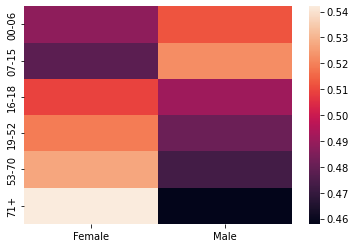
\includegraphics[scale=0.6]{AGE_IM_SEX_IM_Row.png}

Hospitalization Rate Normalized by Age
\end{center}

For full details see the code \verb|CRSS_05_24_22_Crosstabs|.

%%%
\subsection{Handling Data Imbalance and Building Models}

In the Literature Review section we enumerated many methods for dealing with data imbalance, most of which are relevant to our problem.  In the code \verb|CRSS_06_Build_Model_01_15_22.ipynb| we implemented these methods.  We tried all of them, individually and in combinations, to see which combinations of methods give the most effective model.  

\begin{itemize}
	\item Ensure that the training and test sets have the same proportion of positive and negative class samples
	\item Tomek Links, both once and twice
	\item Balanced Metrics
	\begin{itemize}
		\item Balanced Accuracy
		\item Balanced F1
		\item Balanced Precision
	\end{itemize}
	\item Loss Functions
	\begin{itemize}
		\item $\alpha$-weighted Binary Crossentropy
		\item Focal Loss
	\end{itemize}
	\item Model Algorithms
	\begin{itemize}
		\item Keras Simple Neural Network
		\item AdaBoost Classifier
		\item Balanced Bagging Classifier
		\item Balanced Random Forest Classifier
	\end{itemize}
\end{itemize}




%%%
\subsection{Model Building}

To build our model, we chose the Keras/Tensorflow \citep{chollet2015keras} library over scikit-learn \citep{scikit-learn} because of the ease of writing a custom loss function, although we did use the sklearn library for many data preparation functions.  

Since our focus is on levels of data availability and handling data imbalance, we did not build a sophisticated model.  We adapted the model from the Tensorflow tutorial on imbalanced data, which uses credit card fraud detection as its application, but works very similarly. \citep{Tensorflow_Imbalanced_Data}


\input{Methods_Model_Evaluation}
%%%
\subsection{Louisiana Data}

%%%%% Results
\section{Results}

%%%%% Conclusions
\section{Conclusions}

%%%%%
\section{Discussion}

%%%%% Future Work
\section{Future Work}

%%%%%
\section*{Funding Statement}

%%%%% Conflict of Interest
\section*{Conflict of Interest}

The authors have no relevant financial or non-financial interests to disclose.

%%%%% Acknowledgements
\section*{Acknowledgements}

George Broussard contributed to this work in the NSF Research Experiences for Undergraduates program.

%%%%% Data Availability
\section*{Data Availability}

The CRSS data is publicly available at the link in the references.  The Louisiana crash data is not publicly available.  

%%%%% Technical Paper
\section*{Technical Paper}

The technical paper with more detail and the code used for the CRSS data can be found at the corresponding author's GitHub page, \url{https://www.github.com/bburkman}.



\begin{comment}
% Figure
\begin{figure}[<options>]
	\centering
		\includegraphics[<options>]{}
	  \caption{}\label{fig1}
\end{figure}


\begin{table}[<options>]
\caption{}\label{tbl1}
\begin{tabular*}{\tblwidth}{@{}LL@{}}
\toprule
  &  \\ % Table header row
\midrule
 & \\
 & \\
 & \\
 & \\
\bottomrule
\end{tabular*}
\end{table}
\end{comment}

% Uncomment and use as the case may be
%\begin{theorem} 
%\end{theorem}

% Uncomment and use as the case may be
%\begin{lemma} 
%\end{lemma}

%% The Appendices part is started with the command \appendix;
%% appendix sections are then done as normal sections
%% \appendix

\section{}\label{}

% To print the credit authorship contribution details
\printcredits

%% Loading bibliography style file
%\bibliographystyle{model1-num-names}
\bibliographystyle{cas-model2-names}

% Loading bibliography database
\bibliography{Paper_Summer_2022.bib}


\begin{comment}
% Biography
\bio{}
% Here goes the biography details.
\endbio

\bio{pic1}
% Here goes the biography details.
\endbio
\end{comment}

\end{document}

